
%% bare_conf.tex
%% V1.4b
%% 2015/08/26
%% by Michael Shell
%% See:
%% http://www.michaelshell.org/
%% for current contact information.
%%
%% This is a skeleton file demonstrating the use of IEEEtran.cls
%% (requires IEEEtran.cls version 1.8b or later) with an IEEE
%% conference paper.
%%
%% Support sites:
%% http://www.michaelshell.org/tex/ieeetran/
%% http://www.ctan.org/pkg/ieeetran
%% and
%% http://www.ieee.org/

%%*************************************************************************
%% Legal Notice:
%% This code is offered as-is without any warranty either expressed or
%% implied; without even the implied warranty of MERCHANTABILITY or
%% FITNESS FOR A PARTICULAR PURPOSE! 
%% User assumes all risk.
%% In no event shall the IEEE or any contributor to this code be liable for
%% any damages or losses, including, but not limited to, incidental,
%% consequential, or any other damages, resulting from the use or misuse
%% of any information contained here.
%%
%% All comments are the opinions of their respective authors and are not
%% necessarily endorsed by the IEEE.
%%
%% This work is distributed under the LaTeX Project Public License (LPPL)
%% ( http://www.latex-project.org/ ) version 1.3, and may be freely used,
%% distributed and modified. A copy of the LPPL, version 1.3, is included
%% in the base LaTeX documentation of all distributions of LaTeX released
%% 2003/12/01 or later.
%% Retain all contribution notices and credits.
%% ** Modified files should be clearly indicated as such, including  **
%% ** renaming them and changing author support contact information. **
%%*************************************************************************


% *** Authors should verify (and, if needed, correct) their LaTeX system  ***
% *** with the testflow diagnostic prior to trusting their LaTeX platform ***
% *** with production work. The IEEE's font choices and paper sizes can   ***
% *** trigger bugs that do not appear when using other class files.       ***                          ***
% The testflow support page is at:
% http://www.michaelshell.org/tex/testflow/



\documentclass[conference]{IEEEtran}
% Some Computer Society conferences also require the compsoc mode option,
% but others use the standard conference format.
%
% If IEEEtran.cls has not been installed into the LaTeX system files,
% manually specify the path to it like:
% \documentclass[conference]{../sty/IEEEtran}

\RequirePackage[utf8]{inputenc}



% Some very useful LaTeX packages include:
% (uncomment the ones you want to load)


% *** MISC UTILITY PACKAGES ***
%
%\usepackage{ifpdf}
% Heiko Oberdiek's ifpdf.sty is very useful if you need conditional
% compilation based on whether the output is pdf or dvi.
% usage:
% \ifpdf
%   % pdf code
% \else
%   % dvi code
% \fi
% The latest version of ifpdf.sty can be obtained from:
% http://www.ctan.org/pkg/ifpdf
% Also, note that IEEEtran.cls V1.7 and later provides a builtin
% \ifCLASSINFOpdf conditional that works the same way.
% When switching from latex to pdflatex and vice-versa, the compiler may
% have to be run twice to clear warning/error messages.


% *** CITATION PACKAGES ***
\usepackage{cite}
% cite.sty was written by Donald Arseneau
% V1.6 and later of IEEEtran pre-defines the format of the cite.sty package
% \cite{} output to follow that of the IEEE. Loading the cite package will
% result in citation numbers being automatically sorted and properly
% "compressed/ranged". e.g., [1], [9], [2], [7], [5], [6] without using
% cite.sty will become [1], [2], [5]--[7], [9] using cite.sty. cite.sty's
% \cite will automatically add leading space, if needed. Use cite.sty's
% noadjust option (cite.sty V3.8 and later) if you want to turn this off
% such as if a citation ever needs to be enclosed in parenthesis.
% cite.sty is already installed on most LaTeX systems. Be sure and use
% version 5.0 (2009-03-20) and later if using hyperref.sty.
% The latest version can be obtained at:
% http://www.ctan.org/pkg/cite
% The documentation is contained in the cite.sty file itself.






% *** GRAPHICS RELATED PACKAGES ***
%
\ifCLASSINFOpdf
  \usepackage[pdftex]{graphicx}
  % declare the path(s) where your graphic files are
  % \graphicspath{{../pdf/}{../jpeg/}}
  % and their extensions so you won't have to specify these with
  % every instance of \includegraphics
  % \DeclareGraphicsExtensions{.pdf,.jpeg,.png}
\else
  % or other class option (dvipsone, dvipdf, if not using dvips). graphicx
  % will default to the driver specified in the system graphics.cfg if no
  % driver is specified.
  % \usepackage[dvips]{graphicx}
  % declare the path(s) where your graphic files are
  % \graphicspath{{../eps/}}
  % and their extensions so you won't have to specify these with
  % every instance of \includegraphics
  % \DeclareGraphicsExtensions{.eps}
\fi
% graphicx was written by David Carlisle and Sebastian Rahtz. It is
% required if you want graphics, photos, etc. graphicx.sty is already
% installed on most LaTeX systems. The latest version and documentation
% can be obtained at: 
% http://www.ctan.org/pkg/graphicx
% Another good source of documentation is "Using Imported Graphics in
% LaTeX2e" by Keith Reckdahl which can be found at:
% http://www.ctan.org/pkg/epslatex
%
% latex, and pdflatex in dvi mode, support graphics in encapsulated
% postscript (.eps) format. pdflatex in pdf mode supports graphics
% in .pdf, .jpeg, .png and .mps (metapost) formats. Users should ensure
% that all non-photo figures use a vector format (.eps, .pdf, .mps) and
% not a bitmapped formats (.jpeg, .png). The IEEE frowns on bitmapped formats
% which can result in "jaggedy"/blurry rendering of lines and letters as
% well as large increases in file sizes.
%
% You can find documentation about the pdfTeX application at:
% http://www.tug.org/applications/pdftex





% *** MATH PACKAGES ***
%
\usepackage{amsmath}
% A popular package from the American Mathematical Society that provides
% many useful and powerful commands for dealing with mathematics.
%
% Note that the amsmath package sets \interdisplaylinepenalty to 10000
% thus preventing page breaks from occurring within multiline equations. Use:
%\interdisplaylinepenalty=2500
% after loading amsmath to restore such page breaks as IEEEtran.cls normally
% does. amsmath.sty is already installed on most LaTeX systems. The latest
% version and documentation can be obtained at:
% http://www.ctan.org/pkg/amsmath





% *** SPECIALIZED LIST PACKAGES ***
%
%\usepackage{algorithmic}
% algorithmic.sty was written by Peter Williams and Rogerio Brito.
% This package provides an algorithmic environment fo describing algorithms.
% You can use the algorithmic environment in-text or within a figure
% environment to provide for a floating algorithm. Do NOT use the algorithm
% floating environment provided by algorithm.sty (by the same authors) or
% algorithm2e.sty (by Christophe Fiorio) as the IEEE does not use dedicated
% algorithm float types and packages that provide these will not provide
% correct IEEE style captions. The latest version and documentation of
% algorithmic.sty can be obtained at:
% http://www.ctan.org/pkg/algorithms
% Also of interest may be the (relatively newer and more customizable)
% algorithmicx.sty package by Szasz Janos:
% http://www.ctan.org/pkg/algorithmicx




% *** ALIGNMENT PACKAGES ***
%
\usepackage{array}
% Frank Mittelbach's and David Carlisle's array.sty patches and improves
% the standard LaTeX2e array and tabular environments to provide better
% appearance and additional user controls. As the default LaTeX2e table
% generation code is lacking to the point of almost being broken with
% respect to the quality of the end results, all users are strongly
% advised to use an enhanced (at the very least that provided by array.sty)
% set of table tools. array.sty is already installed on most systems. The
% latest version and documentation can be obtained at:
% http://www.ctan.org/pkg/array


% IEEEtran contains the IEEEeqnarray family of commands that can be used to
% generate multiline equations as well as matrices, tables, etc., of high
% quality.




% *** SUBFIGURE PACKAGES ***
%\ifCLASSOPTIONcompsoc
%  \usepackage[caption=false,font=normalsize,labelfont=sf,textfont=sf]{subfig}
%\else
  \usepackage[caption=false,font=footnotesize]{subfig}
%\fi
% subfig.sty, written by Steven Douglas Cochran, is the modern replacement
% for subfigure.sty, the latter of which is no longer maintained and is
% incompatible with some LaTeX packages including fixltx2e. However,
% subfig.sty requires and automatically loads Axel Sommerfeldt's caption.sty
% which will override IEEEtran.cls' handling of captions and this will result
% in non-IEEE style figure/table captions. To prevent this problem, be sure
% and invoke subfig.sty's "caption=false" package option (available since
% subfig.sty version 1.3, 2005/06/28) as this is will preserve IEEEtran.cls
% handling of captions.
% Note that the Computer Society format requires a larger sans serif font
% than the serif footnote size font used in traditional IEEE formatting
% and thus the need to invoke different subfig.sty package options depending
% on whether compsoc mode has been enabled.
%
% The latest version and documentation of subfig.sty can be obtained at:
% http://www.ctan.org/pkg/subfig




% *** FLOAT PACKAGES ***
%
%\usepackage{fixltx2e}
% fixltx2e, the successor to the earlier fix2col.sty, was written by
% Frank Mittelbach and David Carlisle. This package corrects a few problems
% in the LaTeX2e kernel, the most notable of which is that in current
% LaTeX2e releases, the ordering of single and double column floats is not
% guaranteed to be preserved. Thus, an unpatched LaTeX2e can allow a
% single column figure to be placed prior to an earlier double column
% figure.
% Be aware that LaTeX2e kernels dated 2015 and later have fixltx2e.sty's
% corrections already built into the system in which case a warning will
% be issued if an attempt is made to load fixltx2e.sty as it is no longer
% needed.
% The latest version and documentation can be found at:
% http://www.ctan.org/pkg/fixltx2e


\usepackage{stfloats}
% stfloats.sty was written by Sigitas Tolusis. This package gives LaTeX2e
% the ability to do double column floats at the bottom of the page as well
% as the top. (e.g., "\begin{figure*}[!b]" is not normally possible in
% LaTeX2e). It also provides a command:
%\fnbelowfloat
% to enable the placement of footnotes below bottom floats (the standard
% LaTeX2e kernel puts them above bottom floats). This is an invasive package
% which rewrites many portions of the LaTeX2e float routines. It may not work
% with other packages that modify the LaTeX2e float routines. The latest
% version and documentation can be obtained at:
% http://www.ctan.org/pkg/stfloats
% Do not use the stfloats baselinefloat ability as the IEEE does not allow
% \baselineskip to stretch. Authors submitting work to the IEEE should note
% that the IEEE rarely uses double column equations and that authors should try
% to avoid such use. Do not be tempted to use the cuted.sty or midfloat.sty
% packages (also by Sigitas Tolusis) as the IEEE does not format its papers in
% such ways.
% Do not attempt to use stfloats with fixltx2e as they are incompatible.
% Instead, use Morten Hogholm'a dblfloatfix which combines the features
% of both fixltx2e and stfloats:
%
%\usepackage{dblfloatfix}
% The latest version can be found at:
% http://www.ctan.org/pkg/dblfloatfix




% *** PDF, URL AND HYPERLINK PACKAGES ***
%
\usepackage{url}
% url.sty was written by Donald Arseneau. It provides better support for
% handling and breaking URLs. url.sty is already installed on most LaTeX
% systems. The latest version and documentation can be obtained at:
% http://www.ctan.org/pkg/url
% Basically, \url{my_url_here}.




% *** Do not adjust lengths that control margins, column widths, etc. ***
% *** Do not use packages that alter fonts (such as pslatex).         ***
% There should be no need to do such things with IEEEtran.cls V1.6 and later.
% (Unless specifically asked to do so by the journal or conference you plan
% to submit to, of course. )


% correct bad hyphenation here
\hyphenation{op-tical net-works semi-conduc-tor}


\begin{document}
%
% paper title
% Titles are generally capitalized except for words such as a, an, and, as,
% at, but, by, for, in, nor, of, on, or, the, to and up, which are usually
% not capitalized unless they are the first or last word of the title.
% Linebreaks \\ can be used within to get better formatting as desired.
% Do not put math or special symbols in the title.
\title{An\'alise de tr\'afego de dados \\ por transmiss\~ao sem fio}


% author names and affiliations
% use a multiple column layout for up to three different
% affiliations
%\author{\IEEEauthorblockN{Davi Shinji Mota Kawasaki}
%\IEEEauthorblockA{Engenharia da Computa\c{c}\~ao\\
%Universidade Tecnol\'ogica Federal do Paran\'a\\
%Corn\'elio Proc\'opio/PR 86300-000\\
%Email: davishinjik@gmail.com}
%\and
%\IEEEauthorblockN{Homer Simpson}
%\IEEEauthorblockA{Twentieth Century Fox\\
%Springfield, USA\\
%Email: homer@thesimpsons.com}
%\and
%\IEEEauthorblockN{James Kirk\\ and Montgomery Scott}
%\IEEEauthorblockA{Starfleet Academy\\
%San Francisco, California 96678--2391\\
%Telephone: (800) 555--1212\\
%Fax: (888) 555--1212}}

% conference papers do not typically use \thanks and this command
% is locked out in conference mode. If really needed, such as for
% the acknowledgment of grants, issue a \IEEEoverridecommandlockouts
% after \documentclass

% for over three affiliations, or if they all won't fit within the width
% of the page, use this alternative format:
% 
\author{\IEEEauthorblockN{Davi Shinji Mota Kawasaki\IEEEauthorrefmark{1},
Higor Augusto Bassi Rozan\IEEEauthorrefmark{2},
\\João Vitor Bertoncini\IEEEauthorrefmark{3}, 
Vinícius Drago Romano\IEEEauthorrefmark{4}}
\IEEEauthorblockA{\IEEEauthorrefmark{1}Engenharia da Computação, Cornélio Procópio/PR 86300-00\\ Email: kawasaki@alunos.utfpr.edu.br}
\IEEEauthorblockA{\IEEEauthorrefmark{2}Engenharia da Computação, Cornélio Procópio/PR\\
Email: higorb.rozan@hotmail.com}
\IEEEauthorblockA{\IEEEauthorrefmark{3}Engenharia da Computação, Cornélio Procópio/PR 86300-000\\
Email: joaobertoncini@alunos.utfpr.edu.br}
\IEEEauthorblockA{\IEEEauthorrefmark{4}Engenharia da Computação, Cornélio Procópio/PR 86300-000\\ Email: romano@alunos.utfpr.edu.br}}




% use for special paper notices
%\IEEEspecialpapernotice{(Invited Paper)}




% make the title area
\maketitle

% As a general rule, do not put math, special symbols or citations
% in the abstract
%\begin{abstract}
%The abstract goes here.
%\end{abstract}

% no keywords




% For peer review papers, you can put extra information on the cover
% page as needed:
% \ifCLASSOPTIONpeerreview
% \begin{center} \bfseries EDICS Category: 3-BBND \end{center}
% \fi
%
% For peerreview papers, this IEEEtran command inserts a page break and
% creates the second title. It will be ignored for other modes.
\IEEEpeerreviewmaketitle



\section{Introdução}
% no \IEEEPARstart
O objetivo desse documento \'e apresentar a proposta de trabalho referente a an\'alise de tr\'afego de dados por meio de transmiss\~ao sem fio.
O enfoque ser\'a o envio de dados por meio de componentes eletr\^onicos - principalmente a plataforma aberta \textit{Arduino} e \textit{shields} complementares - para an\'alise e tratamento, de forma que a verifica\c{c}\~ao dos sinais dos pacotes seja analisada e modulada para poss\'iveis corre\c{c}\~ao de erros, os quais s\~ao provenientes, por exemplo, de interfer\^encia eletromagn\'etica, dist\^ancias de alcance e obst\'aculos de materiais \cite{ciscoRfProblems}.
Sendo assim, no t\'opico seguinte as propostas desse projeto ser\~ao apresentadas no maior detalhe.

%\hfill mds
 
%\hfill August 26, 2015

\section{Fundamentação Teórica}

\subsection{Coração e Eletrocardiogramas (ECG)}

O coração consiste em um órgão localizado atrás da caixa toráxica, na parte central do peito e entre o pulmão direito e esquerdo \cite{nih2011}. Sua função consiste no batimento ou contração para bombeamento do sangue para todo o corpo por meio de um sistema de vasos sanguíneos \cite{gray1979}.
Antes de qualquer tratamento de dados em transmiss\~oes sem fio, tem-se como o objetivo realizar a conex\~ao dos m\'odulos de r\'adio frequ\^encia com as plataformas abertas \textit{Arduino}. O trabalho visa utilizar dois m\'odulos transceptores \textit{nRF24L01} de 2.4GHz e dois \textit{shields} de \textit{Arduino} UNO, de forma que os m\'odulos transceptores s\~ao conectados as portas seriais dos \textit{Arduinos} UNO por meio de 8 portas, comunicando-se com o \textit{shield} em quest\~ao por meio do protocolo SPI (Serial Peripheral Interface) e por meio da modula\c{c}\~ao GFSK (\textit{Gaussian Frequency Shift Keying}) do sinal, sendo esse \'ultimo um m\'etodo de invers\~ao da frequ\^encia por meio de um filtro Gaussiano \cite{pdsGFSKModulation} j\'a incluso no dispositivo eletr\^onico. Por ser um transceptor, esses m\'odulos utilizados permitem a comunica\c{c}\~ao \textit{full-duplex}, pois permitem a transmiss\~ao e a recep\c{c}\~ao durante o mesmo per\'iodo de tempo \cite{datasheetNRF24L01}. A representa\c{c}\~ao do diagrama de bloco do transceptor utilizado, com entradas (conectadas ao protocolo SPI), controle de r\'adio, filtros e modulador/demodulador utilizados, podem ser visualizadas na figura \ref{diagramaNrf24l01}.

\begin{figure}[!b]
\centering
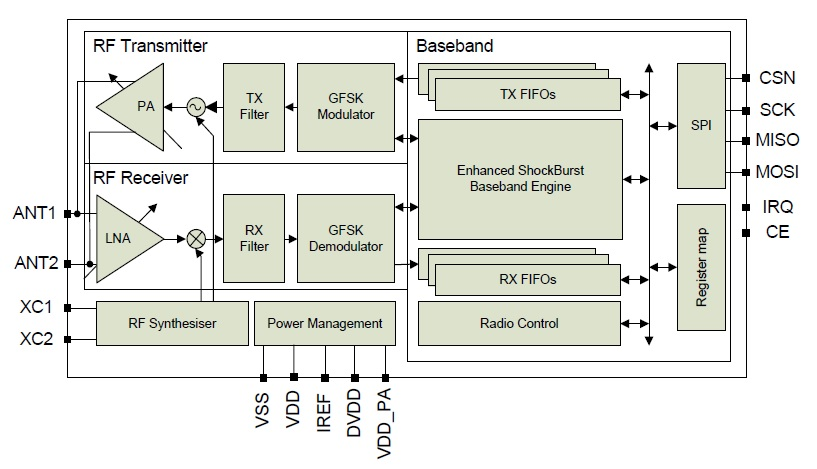
\includegraphics[width=3in]{diagramanrf24l01}
\caption{Diagrama representativo de bloco do m\'odulo nRF24L01.}
\label{diagramaNrf24l01}
\end{figure}

Ap\'os a conex\~ao dos m\'odulos com os \textit{Arduinos}, pretende-se realizar a comunica\c{c}\~ao entre os m\'odulos por meio de uma biblioteca/driver chamado RF24, dado que o mesmo j\'a possui m\'etodos prontos de atua\c{c}\~ao de pot\^encia, taxas de transmiss\~ao, e at\'e mesmo de estabelecimento de uma topologia de rede \cite{driverRF24}.

Por fim, com a obten\c{c}\~ao da conex\~ao e transmiss\~ao de dados sendo realizada efetivamente, os dados - inclusos em um arquivo \textit{txt} - ser\~ao enviados para uma plataforma de tratamento de dados, que ser\'a apresentada no subt\'opico a seguir.

\subsection{Arritmias}

Para o tratamento estat\'istico das informa\c{c}\~oes de transmiss\~ao, ser\'a utilizada a linguagem \textit{Python}, na sua vers\~ao 2.7. Para a conex\~ao com o \textit{Arduino}, ser\'a utilizado o m\'odulo \textit{Pyserial} 3.0.1, que possui m\'etodos para a comunica\c{c}\~ao da porta serial com a placa - seja do \textit{Arduino} para o \textit{Python} como a transmiss\~ao inversa. No c\'odigo fonte gerado para o \textit{Arduino}, s\~ao utilizados m\'etodos que reproduzem as informa\c{c}\~oes na porta serial. A \textit{Pyserial} \'e respons\'avel pela identifica\c{c}\~ao de todos os dados impressos via porta serial, no quais s\~ao armazenados em vetores. O objetivo final dessa proposta \'e a conex\~ao correta e completa entre os \textit{Arduinos} de TX e RX (transmiss\~ao e recep\c{c}\~ao, respectivamente) e o \textit{Python}, de forma que o pr\'oximo t\'opico - Transmiss\~ao e Tratamento de Sinais - seja realizado com sucesso.

\subsection{Processamento do Sinal com \textit{Wavelets}}
Com os dados obtidos e transmitidos corretamente para o \textit{Python}, al\'em de usar os m\'odulos \textit{SciPy} e \textit{MatPlotLib}, tem-se a inten\c{c}\~ao de gerar gr\'aficos estat\'isticos sobre a transmiss\~ao dos pacotes e os sinais transmitidos \cite{pythonPSV}. A partir dos valores obtidos e os gr\'aficos representativos, pretende-se verificar poss\'iveis taxas de erros na transmiss\~ao, perdas de pacotes e at\'e varia\c{c}\~oes na estabilidade de conex\~ao segundo os mesmo t\'opicos apresentados na introdu\c{c}\~ao desse trabalho \cite{ciscoRfProblems}.

A partir dessas propostas, o projeto pretende seguir uma linha de cronograma segundo o t\'opico seguinte, utilizando como ferramenta de gerenciamento de projetos o \textit{Trello}.

\subsection{Classificação de Sinais}
Com os dados obtidos e transmitidos corretamente para o \textit{Python}, al\'em de usar os m\'odulos \textit{SciPy} e \textit{MatPlotLib}, tem-se a inten\c{c}\~ao de gerar gr\'aficos estat\'isticos sobre a transmiss\~ao dos pacotes e os sinais transmitidos \cite{pythonPSV}. A partir dos valores obtidos e os gr\'aficos representativos, pretende-se verificar poss\'iveis taxas de erros na transmiss\~ao, perdas de pacotes e at\'e varia\c{c}\~oes na estabilidade de conex\~ao segundo os mesmo t\'opicos apresentados na introdu\c{c}\~ao desse trabalho \cite{ciscoRfProblems}.

A partir dessas propostas, o projeto pretende seguir uma linha de cronograma segundo o t\'opico seguinte, utilizando como ferramenta de gerenciamento de projetos o \textit{Trello}.

\subsection{Redes Neurais Artificiais}
Com os dados obtidos e transmitidos corretamente para o \textit{Python}, al\'em de usar os m\'odulos \textit{SciPy} e \textit{MatPlotLib}, tem-se a inten\c{c}\~ao de gerar gr\'aficos estat\'isticos sobre a transmiss\~ao dos pacotes e os sinais transmitidos \cite{pythonPSV}. A partir dos valores obtidos e os gr\'aficos representativos, pretende-se verificar poss\'iveis taxas de erros na transmiss\~ao, perdas de pacotes e at\'e varia\c{c}\~oes na estabilidade de conex\~ao segundo os mesmo t\'opicos apresentados na introdu\c{c}\~ao desse trabalho \cite{ciscoRfProblems}.

A partir dessas propostas, o projeto pretende seguir uma linha de cronograma segundo o t\'opico seguinte, utilizando como ferramenta de gerenciamento de projetos o \textit{Trello}.

% An example of a floating figure using the graphicx package.
% Note that \label must occur AFTER (or within) \caption.
% For figures, \caption should occur after the \includegraphics.
% Note that IEEEtran v1.7 and later has special internal code that
% is designed to preserve the operation of \label within \caption
% even when the captionsoff option is in effect. However, because
% of issues like this, it may be the safest practice to put all your
% \label just after \caption rather than within \caption{}.
%
% Reminder: the "draftcls" or "draftclsnofoot", not "draft", class
% option should be used if it is desired that the figures are to be
% displayed while in draft mode.
%
%\begin{figure}[!b]
%\centering
%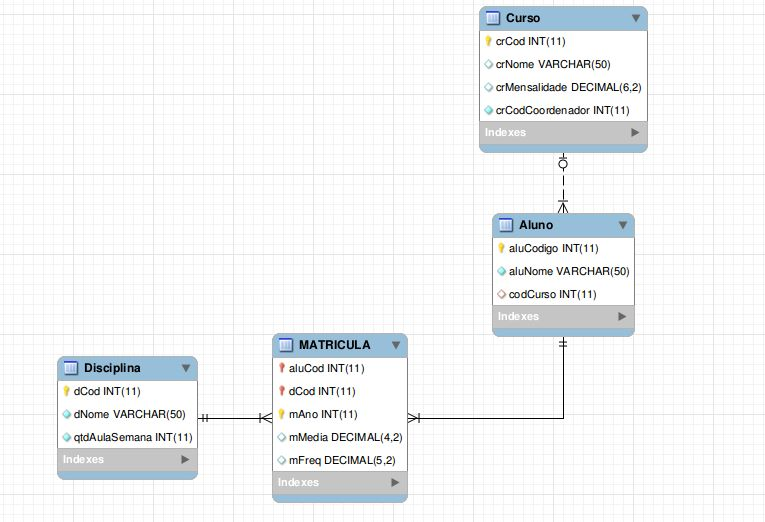
\includegraphics[width=2.5in]{myfigure}
% where an .eps filename suffix will be assumed under latex, 
% and a .pdf suffix will be assumed for pdflatex; or what has been declared
% via \DeclareGraphicsExtensions.
%\caption{Simulation results for the network.}
%\label{fig_sim}
%\end{figure}

% Note that the IEEE typically puts floats only at the top, even when this
% results in a large percentage of a column being occupied by floats.


% An example of a double column floating figure using two subfigures.
% (The subfig.sty package must be loaded for this to work.)
% The subfigure \label commands are set within each subfloat command,
% and the \label for the overall figure must come after \caption.
% \hfil is used as a separator to get equal spacing.
% Watch out that the combined width of all the subfigures on a 
% line do not exceed the text width or a line break will occur.
%
%\begin{figure*}[!b]
%\centering
%\subfloat[Case I]{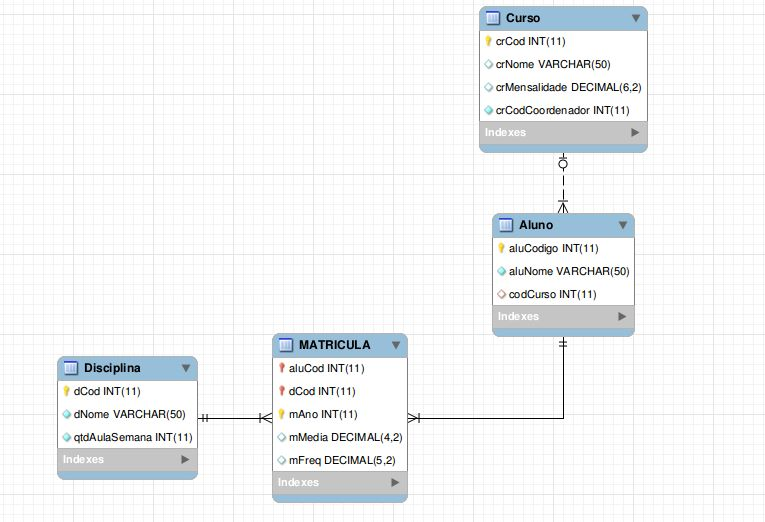
\includegraphics[width=2.5in]{box}%
%\label{fig_first_case}}
%\hfil
%\subfloat[Case II]{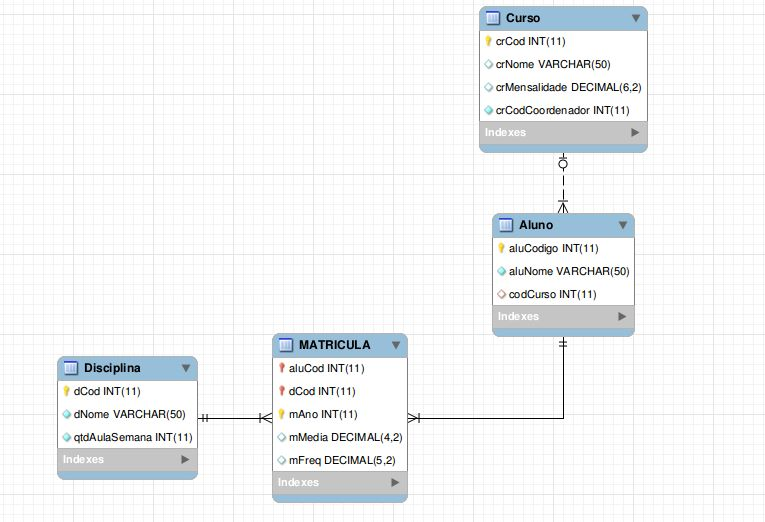
\includegraphics[width=2.5in]{box}%
%\label{fig_second_case}}
%\caption{Simulation results for the network.}
%\label{fig_sim}
%\end{figure*}
%
% Note that often IEEE papers with subfigures do not employ subfigure
% captions (using the optional argument to \subfloat[]), but instead will
% reference/describe all of them (a), (b), etc., within the main caption.
% Be aware that for subfig.sty to generate the (a), (b), etc., subfigure
% labels, the optional argument to \subfloat must be present. If a
% subcaption is not desired, just leave its contents blank,
% e.g., \subfloat[].


% Note that the IEEE does not put floats in the very first column
% - or typically anywhere on the first page for that matter. Also,
% in-text middle ("here") positioning is typically not used, but it
% is allowed and encouraged for Computer Society conferences (but
% not Computer Society journals). Most IEEE journals/conferences use
% top floats exclusively. 
% Note that, LaTeX2e, unlike IEEE journals/conferences, places
% footnotes above bottom floats. This can be corrected via the
% \fnbelowfloat command of the stfloats package.


\section{Cronograma}

O cronograma proposto para esse trabalho de an\'alise de tr\'afego de dados por transmiss\~ao sem fio usando RF (r\'adio frequ\^encia) tem um prazo de aproximadamente 12 semanas de trabalho, come\c{c}ando na \'ultima semana de mar\c{c}o e terminando na pen\'ultima semana de julho (28 de mar\c{c}o a 21 de junho). O trabalho consistir\'a de cerca de 8 semanas de pr\'atica e v\'arios testes envolvendo os m\'odulos RF, enquanto possuir\'a cerca de 6 semanas de estudo envolvendo tratamento de dados e sinais, os quais v\~ao estar presentes nos testes - ressaltando que duas dessas semanas ser\~ao conjuntas com testes de tratamento dos sinais obtidos. Al\'em disso, ser\'a destinada duas semanas a reda\c{c}\~ao exclusiva do artigo final previamente determinado, o qual ocorrer\'a nas semanas do dia 05 a 19 de junho.

Por fim, a pretens\~ao de temas a serem tratadas em cada semana pode ser melhor ilustrada na tabela \ref{table:cronogramaProjeto}.

% An example of a floating table. Note that, for IEEE style tables, the
% \caption command should come BEFORE the table and, given that table
% captions serve much like titles, are usually capitalized except for words
% such as a, an, and, as, at, but, by, for, in, nor, of, on, or, the, to
% and up, which are usually not capitalized unless they are the first or
% last word of the caption. Table text will default to \footnotesize as
% the IEEE normally uses this smaller font for tables.
% The \label must come after \caption as always.
%

\renewcommand\tablename{TABELA}
\begin{table}[!t]
%% increase table row spacing, adjust to taste
\renewcommand{\arraystretch}{1.3}
% if using array.sty, it might be a good idea to tweak the value of
% \extrarowheight as needed to properly center the text within the cells
\caption{Cronograma de Temas do Projeto}
\label{table:cronogramaProjeto}
\centering
%% Some packages, such as MDW tools, offer better commands for making tables
%% than the plain LaTeX2e tabular which is used here.
\begin{tabular}{|c|c|}
\hline
Semana 27/03 & Testes de Conex\~ao \textit{Arduino} e m\'odulo RF\\
\hline
Semana 03/04 & Testes de Conex\~ao \textit{Arduino} e \textit{Python}\\
\hline
Semana 10/04 & Proposta + Escrita do c\'odigo de transmiss\~ao\\
\hline
Semana 17/04 & Escrita do c\'odigo de transmiss\~ao + Envio \textit{Python}\\
\hline
Semana 24/04 & Estudo de tratamento de dados (Teoria e \textit{Python})\\
\hline
Semana 08/05 & Testes de c\'odigos + Gera\c{c}\~ao de gr\'aficos\\
\hline
Semana 15/05 & Apresenta\c{c}\~ao do Andamento + Gera\c{c}\~ao de gr\'aficos\\
\hline
Semana 22/05 & Estudo de tratamento de dados (Teoria e \textit{Python})\\
\hline
Semana 29/05 & Estudo de tratamento de dados + Tratamento de Sinais\\
\hline
Semana 05/06 & Escrita do Artigo + Poss\'iveis modifica\c{c}\~oes\\
\hline
Semana 12/06 & Escrita do Artigo\\
\hline
Semana 19/06 & Apresenta\c{c}\~ao Final\\
\hline
\end{tabular}
\end{table}

\section{Conclus\~ao}
Como apresentado anteriormente, o objetivo desse trabalho \'e realizar n\~ao apenas a conex\~ao entre dois m\'odulos de r\'adio frequ\^encia, mas principalmente realizar a an\'alise dos pacotes e dados enviados, verificando poss\'iveis erros e perdas. Nesse quesito, o projeto deve apresentar, em sua entrega e apresenta\c{c}\~ao, a transmiss\~ao de pacotes de dados em tempo real e a gera\c{c}\~ao de gr\'aficos e dados estat\'isticos que possam ilustrar a situa\c{c}\~ao real dessa transfer\^encia sob diferentes aspectos do meio.

Caso seja poss\'ivel, o projeto tamb\'em pode visar o tratamento desses dados diretamente nos atuadores, visualizando poss\'iveis situa\c{c}\~oes que possam corrigir e inibir erros e atenua\c{c}\~oes que influenciam e impedem o tr\'afego dos dados da melhor maneira poss\'ivel.

O projeto tamb\'em poder\'a trabalhar com os seguintes artigos, dependendo do n\'ivel de desenvolvimento do estudo: \cite{performanceAnalysisNRF24L01}, \cite{efficientRFPowerTransfer} e \cite{selectionOpticalWavelengthDataTransmission}.


% conference papers do not normally have an appendix


% use section* for acknowledgment
%\section*{Acknowledgment}


%The authors would like to thank...





% trigger a \newpage just before the given reference
% number - used to balance the columns on the last page
% adjust value as needed - may need to be readjusted if
% the document is modified later
%\IEEEtriggeratref{8}
% The "triggered" command can be changed if desired:
%\IEEEtriggercmd{\enlargethispage{-5in}}

% references section

% can use a bibliography generated by BibTeX as a .bbl file
% BibTeX documentation can be easily obtained at:
% http://mirror.ctan.org/biblio/bibtex/contrib/doc/
% The IEEEtran BibTeX style support page is at:
% http://www.michaelshell.org/tex/ieeetran/bibtex/
\def\refname{Refer\^encias}
\bibliographystyle{IEEEtran}
% argument is your BibTeX string definitions and bibliography database(s)
\bibliography{IEEEabrv}
%
% <OR> manually copy in the resultant .bbl file
% set second argument of \begin to the number of references
% (used to reserve space for the reference number labels box)
% \begin{thebibliography}{1}

%\bibitem{IEEEhowto:kopka}
%H.~Kopka and P.~W. Daly, \emph{A Guide to \LaTeX}, 3rd~ed.\hskip 1em plus
%  0.5em minus 0.4em\relax Harlow, England: Addison-Wesley, 1999.

% \end{thebibliography}




% that's all folks
\end{document}


